% !TeX root = ../paper.tex
\section{Visualization Approach}
\label{sec:visualization_approach}

In this section, we describe the prerequisites and the design of our proposed visualization approach.

\subsection{Data Model}
\label{sec:visualization_approach/data_model}

\begin{figure}
	\includegraphics[width=\linewidth]{sections/03_visualization_approach/data_model.tikz}
	\caption{TODO}
	\Description{TODO}
	\label{fig:visualization_approach/data_model}
\end{figure}

%For the data source of the visualization, we assume a simple program trace model for object-oriented programs~(\cref{fig:visualization_approach/data_model}).
The data source of our visualization is the program trace of an object-oriented program.
%An object is characterized by its \emph{identity} which distinguishes it from all other objects in the system, its \emph{state} which is represented by its fields such as array elements and instance variables, and its \emph{behavior} which is described by methods that implement the reception of messages~\cite{thiede2023time}.
In this programming paradigm, all behavior is described as \emph{messages} sent from one object to another.
Each object is characterized by its \emph{identity} which distinguishes it from all other objects in the system, its \emph{state} which is represented by its fields such as array elements and instance variables, and its \emph{behavior} which is implemented by methods that are invoked to receive messages~\cite{thiede2023time}.

We assume a minimal data model of the program trace~(\cref{fig:visualization_approach/data_model}):
the \emph{call tree} is represented as a composite structure of \emph{stack frames} each of which specifies a time interval, an invoked method, and a receiver object.
Each \emph{object} is assigned a label, a list of named fields, and a class.
%The value of each \emph{field} can be a reference to another object or a flat string representation.
Each \emph{class} is described through a name and an organizational path in the file or package structure of the software system.
We neglect runtime changes to the state, label, or class membership of objects as well as metaprogramming specifics such as the implementation of classes or methods as objects.
% TODO: we also neglect coroutine, multiple processes, etc. but is this the right place to mention all of that?

\subsection{Visual Mapping}
\label{sec:visualization_approach/mapping}

We describe the design of our visualization and the mapping of parts from the program trace to elements and visual variables of our visualization~(\cref{fig:teaser}).
At the highest level, an animated 2.5 object map is an interactive information landscape that displays objects and their interactions from the program trace.
Users can replay the program trace and watch the activation and interaction of objects.
They can unrestrictedly navigate through the visual scene using their keyboard and pointing devices and view the map from all sides.

\paragraph{Objects}
\label{sec:visualization_approach/mapping/objects}

\begin{figure}
	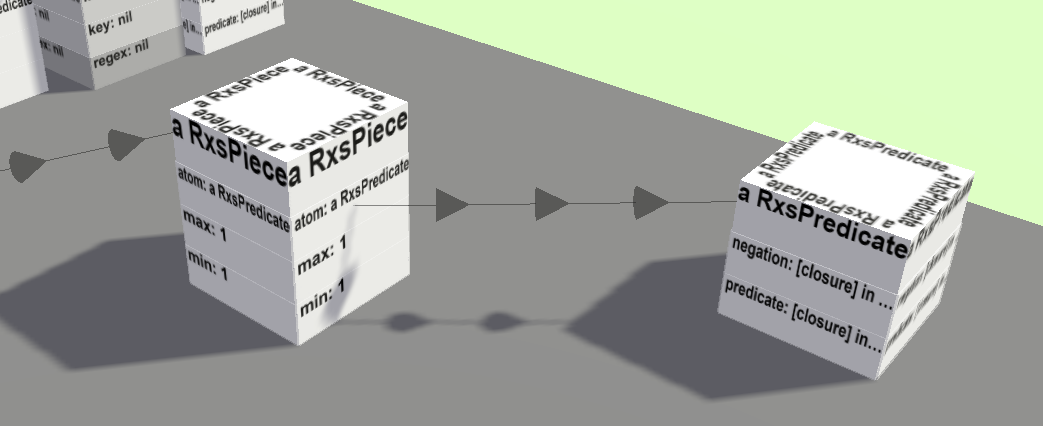
\includegraphics[width=\linewidth]{sections/03_visualization_approach/mapping/objects}
	\caption{TODO}
	\Description{TODO}
	\label{fig:visualization_approach/mapping/objects}
\end{figure}
% TODO: maybe cut better

Each object is represented as a square cuboid \emph{block} entity that displays the label and fields of the object~(\cref{fig:visualization_approach/mapping/objects}).
To maximize legibility from any perspective, the label is repeated on all four sides and in four orientations on the top of the block.
Fields are displayed as \emph{plates} that are arranged in a row-wise uniform-sized grid layout and repeated on each side of the block for better legibility.
References between objects are rendered as \emph{directed arrows} from the closest plate of the referencing field to the closest label of the referenced object's entity.
To indicate the direction of arrows, we place between one and ten evenly distributed \emph{chevrons} on the arrow line; each chevron is displayed as a cone whose direction can be recognized from any perspective.

\paragraph{Object graph}
\label{sec:visualization_approach/mapping/object_graph}

\begin{figure}
	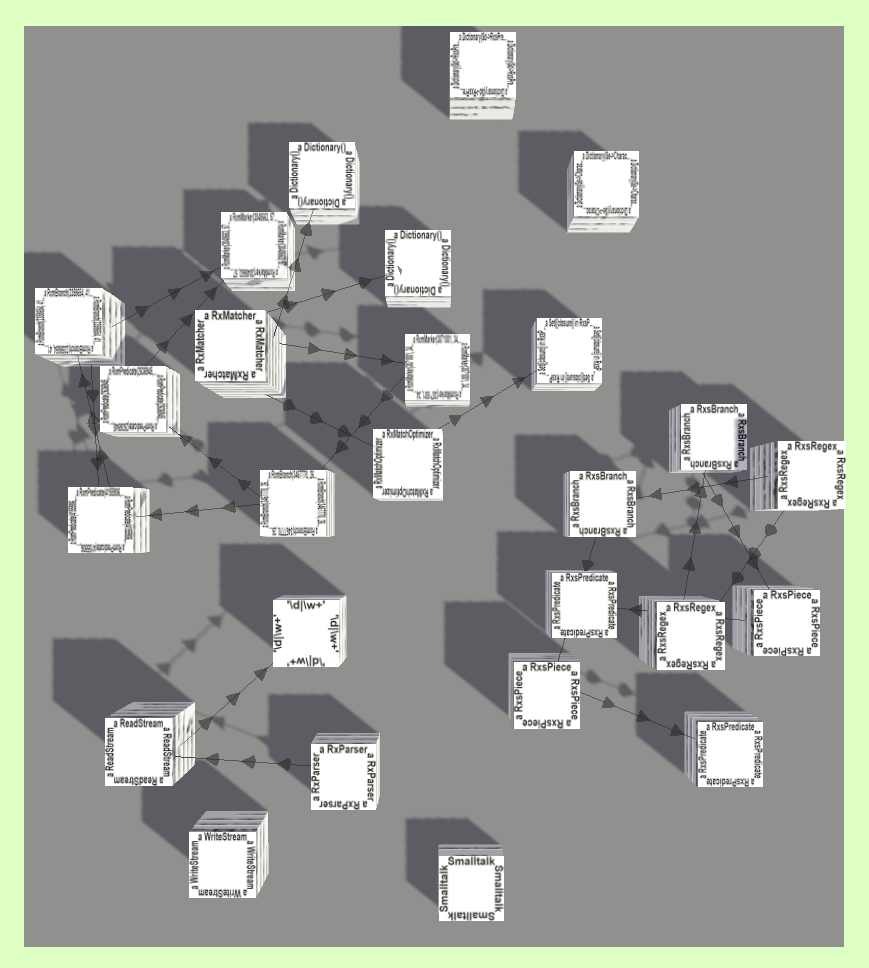
\includegraphics[height=.25\textheight]{sections/03_visualization_approach/mapping/object_graph}
	\caption{TODO}
	\Description{TODO}
	\label{fig:visualization_approach/mapping/object_graph}
\end{figure}
% TODO: maybe highlight object for dragging?
% TODO: how useful is this? you can't read anything.
% TODO: improve figure layout? bundle object_graph and object_behavior in a single figure?

To arrange object blocks in the 2.5D object map, we define a force-directed graph layout~\cite{fruchterman1991graph}.
Between each pair of object blocks $(a, b)$, we apply several \emph{weighted attractive forces} based on the class membership, the organizational proximity of classes, and the references and communication between objects~(\cref{fig:visualization_approach/mapping/object_graph}):

\begin{equation}
	\begin{split}
		F_{\text{class}}(a, b) &= w_{\text{class}}\left(\begin{cases}1, & \text{if $\text{class}(a) = \text{class}(b)$;} \\ 0, & \text{otherwise}.\end{cases}\right) \,, \\
		F_{\text{org}}(a, b) &= w_{\text{org}}\bigl(\text{LCP}\footnotemark\bigl(\text{org}\footnotemark(a), \text{org}(b)\bigr)\bigr) \,, \\
		F_{\text{ref}}(a, b) &= w_{\text{ref}}\left(\left|\bigl\{ (k, v) \in \text{fields}(a) ~\middle\vert~ v = b \bigr\}\right|\right) \,, \\
		F_{\text{comm}}(a, b) &= w_{\text{comm}}\big(\big|\big\{\text{frame }f ~\big\vert \\
			& \hphantom{= w} \text{$f$.receiver} = a \wedge \text{$f$.parent.receiver} = b\big\}\big|\big) \, .
	\end{split}
\end{equation}
\addtocounter{footnote}{-1}
\footnotetext{$\text{LCP}(u, v)$: Largest common prefix of two sequences $u$ and $v$.}
\footnotetext{$\text{org}(o)$: Organizational path to an object $o$'s class (e.g., a file path).}

\begin{table}
	\centering
	\caption{TODO}
	\label{tab:visualization_approach/mapping/object_graph/default_configuration}
	\begin{threeparttable}
		\centering
		{\footnotesize
		% !TeX root = ../../../../paper.tex
{\setlength\tabcolsep{3pt}
\begin{tabular}{cccc c cc}
	\toprule

	\multicolumn{1}{c}{\bold{$w_{\text{class}}$}}	&
	\multicolumn{1}{c}{\bold{$w_{\text{org}}$}}	&
	\multicolumn{1}{c}{\bold{$w_{\text{ref}}$}}	&
	\multicolumn{1}{c}{\bold{$w_{\text{comm}}$}}	&
		&
	\multicolumn{1}{c}{\bold{$w_{\text{repulse}}$}}	&
	\multicolumn{1}{c}{\bold{$w_{\text{center}}$}}	\\

	\midrule

	$0.001$	&
	$F \mapsto 0.005 \left(\log_{10}(F) + 1\right)$	&
	$0.1$	&
	$0.00001$	&
		&
	$0.2$	&
	$0.00142$	\\

	\bottomrule
\end{tabular}}
}
	\end{threeparttable}
\end{table}

In addition to the attractive forces, we define globally weighted \emph{repulsion} and \emph{centripetation} forces on all blocks to control the entropy of the graph, and we define \emph{radial constraints} to avoid collisions between blocks.

We provide an empirical base configuration for all force weights but enable users to override them for specific program traces.
By default, we prioritize reference forces the highest and organizational forces the lowest with a distance of six orders of magnitudes and scale organizational forces logarithmically~(\cref{tab:visualization_approach/mapping/object_graph/default_configuration}).
This configuration fosters a state-centric layout of the object graph while leaving a margin for the characteristic of particular program traces (e.g., their ratio between intrinsic and extrinsic state~\cite[p. 218ff]{gamma1994design}) towards a more dataflow-driven layout. % TODO: does this belong into discussion?
Additionally, users can drag and drop blocks to override the layout.
To reduce response times and maintain an experience of immediacy~\cites[chap. 11]{shneiderman2005designing}{ungar1997debugging}, we render the graph continuously before the force simulation has converged.

\paragraph{Object selection}
\label{sec:visualization_approach/mapping/object_selection}

Usually, even after restricting the object graph to the receivers from the call tree~(\cref{sec:visualization_approach/data_model}), only a small part of it is relevant for comprehending the high-level behavior of a program while many other objects fulfill lower-level implementation details.
In our visualization, we use a filtering system for excluding objects based on their label, class, or organization.
Similarly to the layout configuration~(\lcnameref{sec:visualization_approach/mapping/object_graph}), we provide an empirical default configuration that excludes certain base objects such as collections, booleans, and numbers, but allow users to customize these filters.

\paragraph{Object behavior}
\label{sec:visualization_approach/mapping/object_behavior}

\begin{figure}
	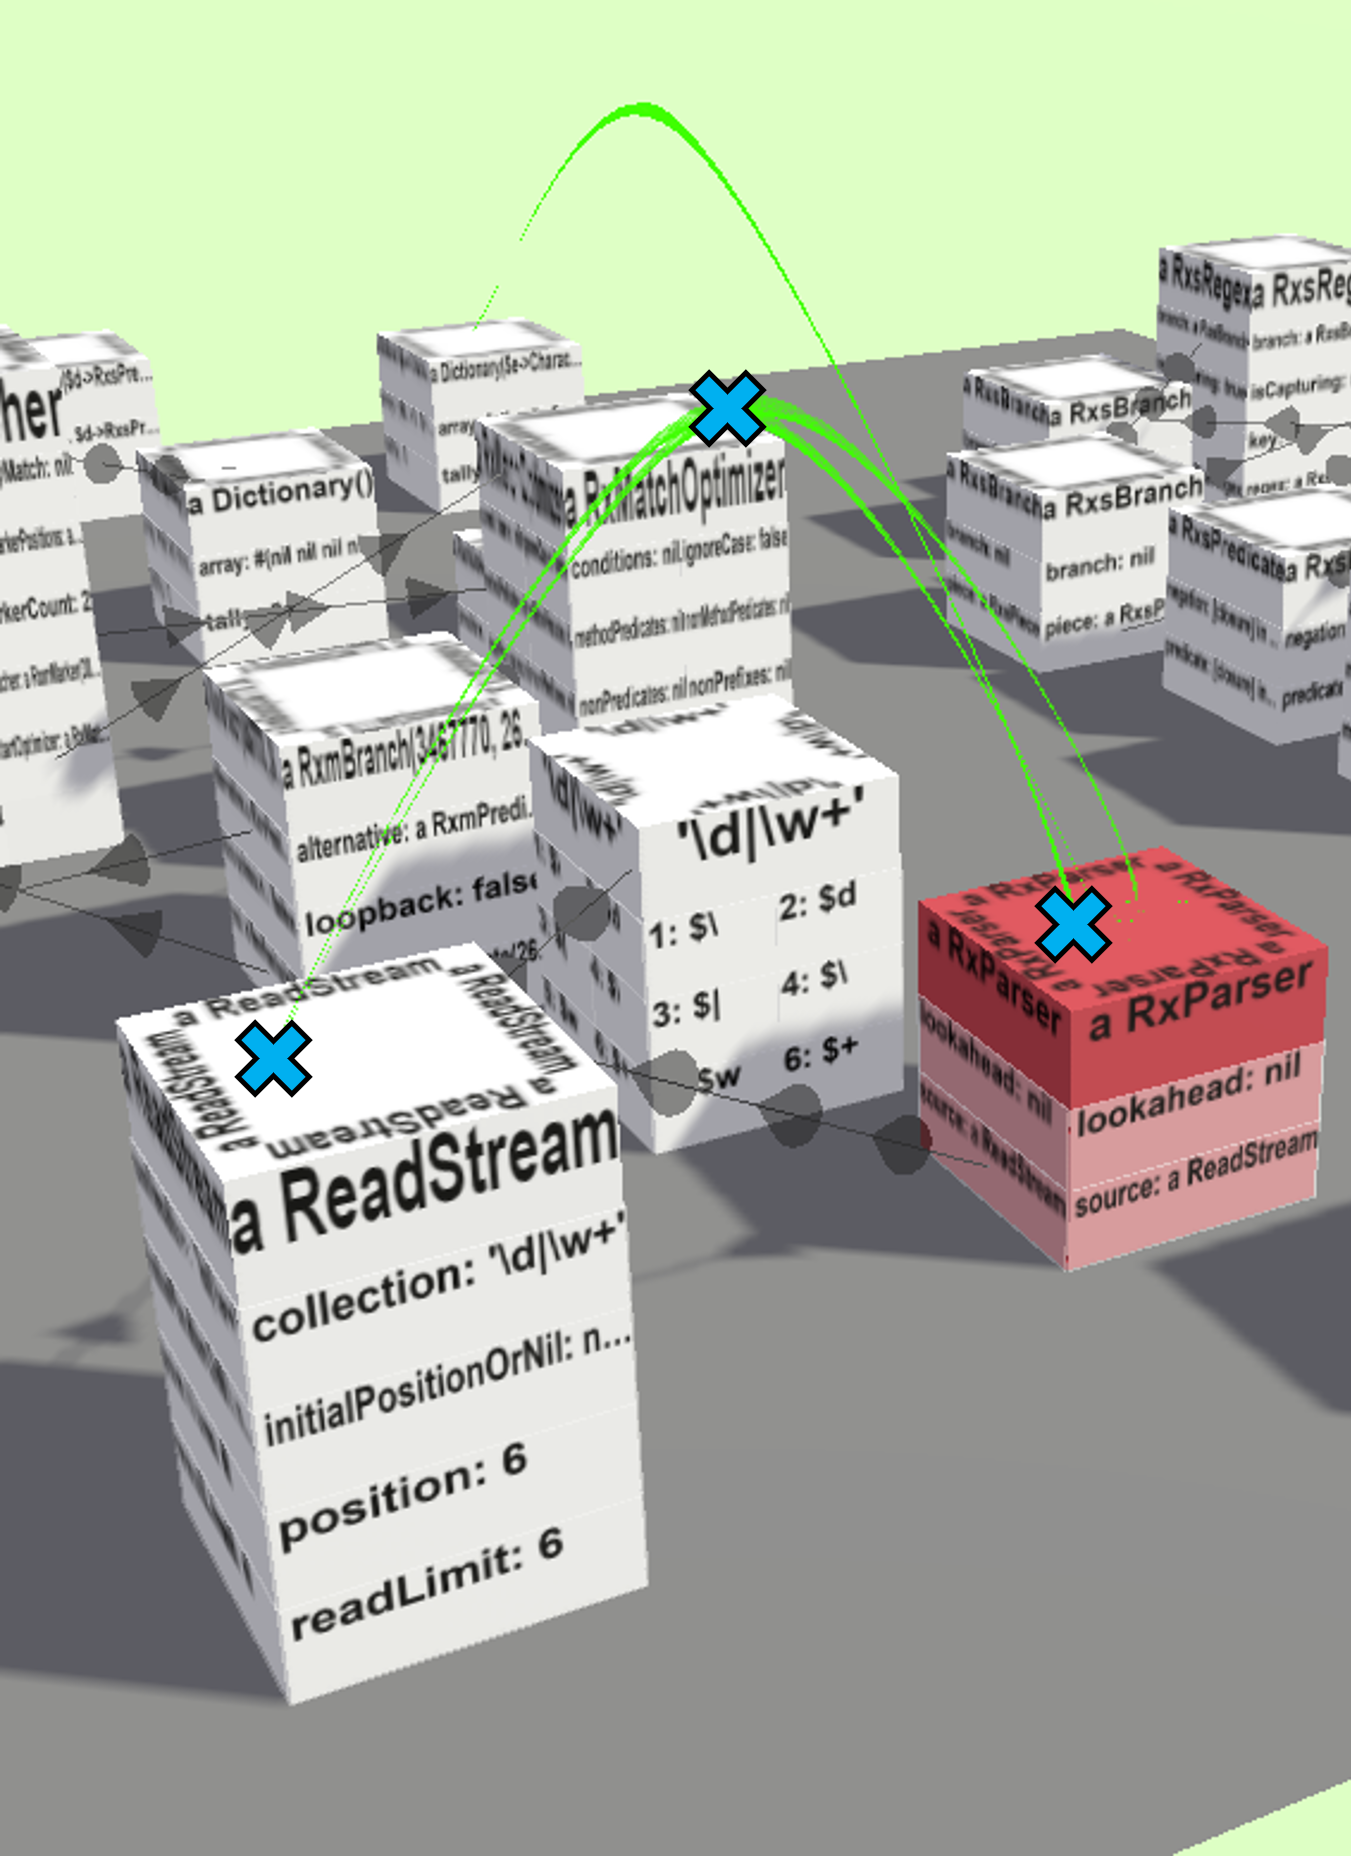
\includegraphics[height=.25\textheight]{sections/03_visualization_approach/mapping/object_behavior}
	\caption{TODO}
	\Description{TODO}
	\label{fig:visualization_approach/mapping/object_behavior}
\end{figure}
% TODO: add different tones of red! maybe change cropping?

The color of each object block displays its recent activity:
\emph{inactive} blocks are colored in a neutral light gray while \emph{active} blocks whose objects have received a message recently are highlighted in a bright red~(\cref{fig:visualization_approach/mapping/object_behavior}).
After the control flow passes on to other objects, blocks linearly fade back to the base color within one second, thus applying a single-hue continuous sequential color scheme by Brewer et al.\footnote{Cynthia Brewer and Mark Harrower. 2013 -- 2021. ColorBrewer: Color Advice for Cartography. Pennsylvania State University. URL: \url{https://colorbrewer2.org/}}

Next to the color coding, a \emph{trail} connects the most recent $k = 15$ object activations to support the delayed observation of short activations and the recognition of exact activation order.
The trail curve is based on a centripetal Catmull-Rom spline~\cite{catmull1974class} whose control points are placed on the top of each relevant block and are alternated with intermediate points between blocks.
Block control points are normally randomized to make multiple activations of the same object distinguishable.
Intermediate control points are vertically elevated to give the curve a wave-like shape that makes activated objects identifiable.
The direction of the trail is displayed by continuously moving it to the next object and applying a linear translucency gradient to fade out the tail of the curve.
% TODO: Somewhere talk about callstack idea? Footnote?

\paragraph{Timeline}
\label{sec:visualization_approach/mapping/timeline}

\begin{figure}
	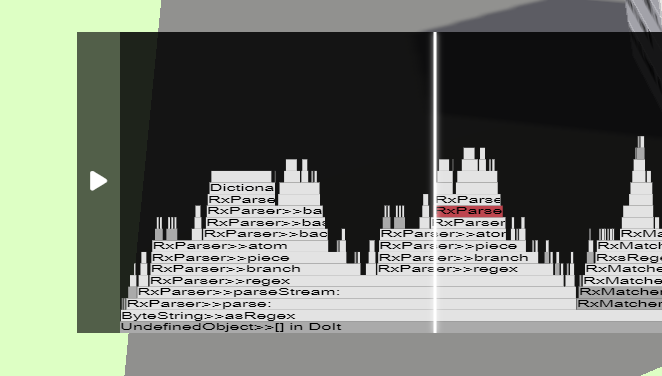
\includegraphics[width=\linewidth]{sections/03_visualization_approach/mapping/timeline}
	\caption{TODO}
	\Description{TODO}
	\label{fig:visualization_approach/mapping/timeline}
\end{figure}
% TODO: change cropping?

The object map integrates a \emph{timeline} overlay at the bottom of the viewport that provides a time-centric navigational aid.
The timeline consists of two widgets stacked on top of each other~(\cref{fig:visualization_approach/mapping/timeline}):
a \emph{player} with a slider and a play/pause button indicates the current point in time of the program trace and allows to control the time and animation state.
Behind the player, a collapsed \emph{flame graph} displays the course of the call stack depth.
Users can resize the timeline to explore the full call tree hierarchy and examine single frames in the flame graph.

Both the flame graph and the object map are interactively connected, i.e., users can hover an object in the map to discover all of its activations in the timeline, or vice versa, they can click on a frame to move the trail in the map to the relevant activation of the object.
Thus, object map and timeline provide two orthogonal means for navigating through the object-oriented program trace with different granularities.
